% Inbuilt themes in beamer
\documentclass[aspectratio=169]{beamer}
\usepackage{graphicx}
% Theme choice:
\usetheme{Madrid}

% Title page details: 
\title{Intro to Labor Economics with Claudia Goldin \\ \vspace{2mm} \large Baltimore Polytechnic Guest Lecture} 
\author{John Green}
\institute{\normalsize Johns Hopkins Economics} % Adjust subtitle
\date{December 2023}

\makeatletter
\setbeamertemplate{footline}
{
  \leavevmode%
  \hbox{%
  \begin{beamercolorbox}[wd=.333333\paperwidth,ht=2.25ex,dp=1ex,center]{author in head/foot}%
    \usebeamerfont{author in head/foot}{Baltimore Polytechnic Guest Lecture}
  \end{beamercolorbox}%
  \begin{beamercolorbox}[wd=.333333\paperwidth,ht=2.25ex,dp=1ex,center]{title in head/foot}%
    \usebeamerfont{title in head/foot}\insertauthor
  \end{beamercolorbox}%
  \begin{beamercolorbox}[wd=.333333\paperwidth,ht=2.25ex,dp=1ex,right]{date in head/foot}%
    \usebeamerfont{date in head/foot}\insertshortdate{}\hspace*{2em}
    \insertframenumber{} / \inserttotalframenumber\hspace*{2ex} 
  \end{beamercolorbox}}%
  \vskip0pt%
}
\makeatother

% Customize headline to display section navigation
\addtoheadtemplate{\insertsectionnavigationhorizontal{\paperwidth}{}{\hfill\hfill}}

% Frames for section introductions
\AtBeginSection[]{
  \begin{frame}
    \frametitle{Outline}
    \tableofcontents[currentsection]
  \end{frame}
}
% Customize footline to display specific elements
% Customize headline and footline to display specific elements

\begin{document}

% Title page
\begin{frame}
    \titlepage 
\end{frame}

% Outline frame
\begin{frame}{Plan for today}

\begin{enumerate}
    \item What is labor economics? 
    \item Claudia Goldin and gender economics
    \item Intro to data analysis
    \item Navigating trade-offs at work
\end{enumerate}

\end{frame}

\section{What is labor economics?}

\begin{frame}{Labor economics}
    \begin{itemize}
        \item Micro-economists broadly study \textit{how decisions are made} at the individual level
        \item Usually falls into two categories:
        \begin{enumerate}
            \item How do firms (companies) make decisions?
            \item How do workers or households make decisions?
        \end{enumerate}
        \item Labor economists focus on the second one, specifically focusing on decisions about:
        \begin{enumerate}
            \item Education
            \item Work
            \item Career
            \item Marriage and family
        \end{enumerate}
    \end{itemize}
\end{frame}

\begin{frame}{Labor economics}
    \begin{itemize}
        \item Labor economists are also often in interested in \textit{how} and \textit{why} different groups of people make different decisions and have different experiences
        \begin{itemize}
            \item ``Heterogeneity'' --- understanding differences!
        \end{itemize}
        \item What tools do we use?
        \begin{itemize}
            \item Theoretical models
            \item Real world data
            \item Statistical analysis
        \end{itemize}
        \item Economics is a \textit{social science} --- we try and make true statements about a very messy world using very messy data. This is not easy!
    \end{itemize}
\end{frame}

\section{Claudia Goldin}

\begin{frame}{Claudia Goldin}
\begin{itemize}
    \item Labor economist at Harvard (and the first tenured female economics professor in that dept.!)
    \item Groundbreaking work (largely) in gender economics, which looks at questions such as:
    \begin{itemize}
        \item Gender wage gap 
        \item Female labor force participation
        \item Child penalty
        \item Much, much more
    \end{itemize}
    \item Innovative use of data, cutting-edge statistical techniques, and history
    \item And recently: \textbf{winner of the 2023 Nobel Prize in economics!}
\end{itemize}
\end{frame}

\begin{frame}{Gender wage gap}
    \begin{itemize}
        \item Goldin's work on the gender wage gap points to:
        \begin{itemize}
            \item Career interruptions
            \item Occupational differences
        \end{itemize}
        \item Shows that controlling for these things shrinks the wage gap, but it \textit{not disappear}
        \begin{itemize}
            \item (What do we mean by ``control''?)
        \end{itemize}
        \item Some natural questions:
        \begin{itemize}
            \item Why might these factors lead to lower wages?
            \item Why might these factors affect men and women differently?
            \item What does it mean to ``control'' for things like career interruptions when understanding gender discrimination?     
        \end{itemize}
    \end{itemize}
\end{frame}

\begin{frame}{Other themes}
    Other areas of work:
    \begin{itemize}
        \item Education decisions and ``human capital''
        \begin{itemize}
            \item Emphasizes the importance of college attainment and the role of increasing female college attendance in improved labor market outcomes
        \end{itemize}
        \item Practical policies
        \begin{itemize}
            \item Has highlighted actual government policies which could promote gender equality: flexible work, affordable childcare, etc.
        \end{itemize}
        \item Historical perspective
        \begin{itemize}
            \item Looks at the long run trajectory of female labor force participation
            \item Will discuss this more at the end!
        \end{itemize}
    \end{itemize}
\end{frame}


\section{Data work}

\begin{frame}{Introduction to data work}
    \begin{itemize}
        \item Most of what the majority of economists do on a day-to-day basis involves writing computer code and analyzing data
        \item Let's have a gentle introduction to this using a \textit{Python} notebook
        \item http://tinyurl.com/polyecon
    \end{itemize}
\end{frame}

\section{Tradeoffs at work}

\begin{frame}{Responding to an increased wage}
    \begin{itemize}
        \item One of Goldin's contributions was to explain how female labor force participation has responded to growing wages
        \item Let's try and understand this in a very simple setting
        \item Suppose you have two choices to make:
        \begin{enumerate}
            \item How much to work
            \item How much to consume
        \end{enumerate}
        \item You enjoy consumption, but you dislike working --- which is the same as saying you enjoy \textit{leisure}, or not working
        \item You need to make a decision about the best combination of work and consumption!
    \end{itemize}
\end{frame}

\begin{frame}{Simple example}
    \begin{itemize}
        \item Suppose you make \$20 an hour, work 40 hours per week, and consume \$800 worth of goods (your whole salary)
        \item Now let's say your wage increases to \$30 per hour. How would you respond?
        \begin{itemize}
            \item What would happen if you worked the same amount?
            \item What would happen if you worked 30 hours per week?
            \item What would happen if you worked 50 hours per week?
        \end{itemize}
    \end{itemize}
\end{frame}

\begin{frame}{Simple example}
    \begin{itemize}
        \item Say your wage increases to \$30 per hour. How would you respond?
        \begin{itemize}
            \item \textbf{What would happen if you worked the same amount?} Consume $40 \times \$30 = \$1200 $
            \item \textbf{What would happen if you worked 30 hours per week?} Consume $30 \times \$30 = \$900 $
            \item \textbf{What would happen if you worked 50 hours per week?} Consume $50 \times \$30 = \$1500 $
        \end{itemize}
        \item No matter what, we are happier to be consuming more!
        \item But, we may be more or less happy with hour of work.
        \item Which is best?
    \end{itemize}
\end{frame}

\begin{frame}{Simple example}
    \begin{itemize}
        \item Which is best? \textbf{We don't know!}
        \item To decide whether to increase our work hours, we need to know if the \textit{decrease} in happiness from the extra 10 hours of work is outweighed by the \textit{increase} in happiness from the extra \$300 of consumption
        \item This depends on individual \textit{preferences}
    \end{itemize}
\end{frame}

\begin{frame}{Income and substitution effects}
    \begin{itemize}
        \item There are two different channels at play here:
        \begin{enumerate}
            \item \textbf{Income effect} is the direct effect of the wage increase: we are wealthier, and so we want to increase our consumption \textbf{and} our leisure
            \item \textbf{Substitution effect} is the indirect effect: because our wage is higher, ``purchasing'' free time (the \textit{opportunity cost}) is relatively more expensive, and so we may want to work more hours and consume more 
        \end{enumerate}
        \item Which of these two channels is stronger?
        \begin{itemize}
            \item We don't know! Need to try and measure from the data
        \end{itemize}
    \end{itemize}
\end{frame}

\begin{frame}{Income and substitution effects}
    \begin{itemize}
        \item This was one of the main contributions for which Goldin won the Nobel Prize
        \item She analyzed the trajectory of women's labor force participation over time to show how the two effects balanced out as wages grew
        \begin{itemize}
            \item Also highlighted the importance of occupational shifts, emergence of white-collar work, etc.
        \end{itemize}
        \item Famous ``u-shaped labor supply curve''
    \end{itemize}
\end{frame}

\begin{frame}{U-shaped supply curve}
    \centering
    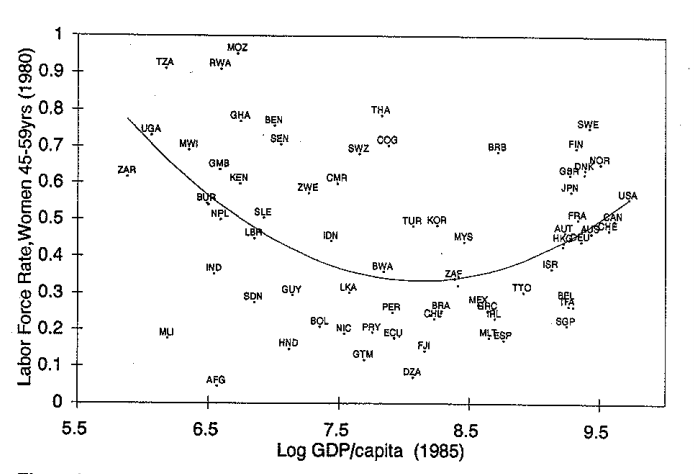
\includegraphics[width = 0.75\textwidth,keepaspectratio]{./figs/ushape.png}
\end{frame}

\begin{frame}{U-shaped supply curve}
    \centering
    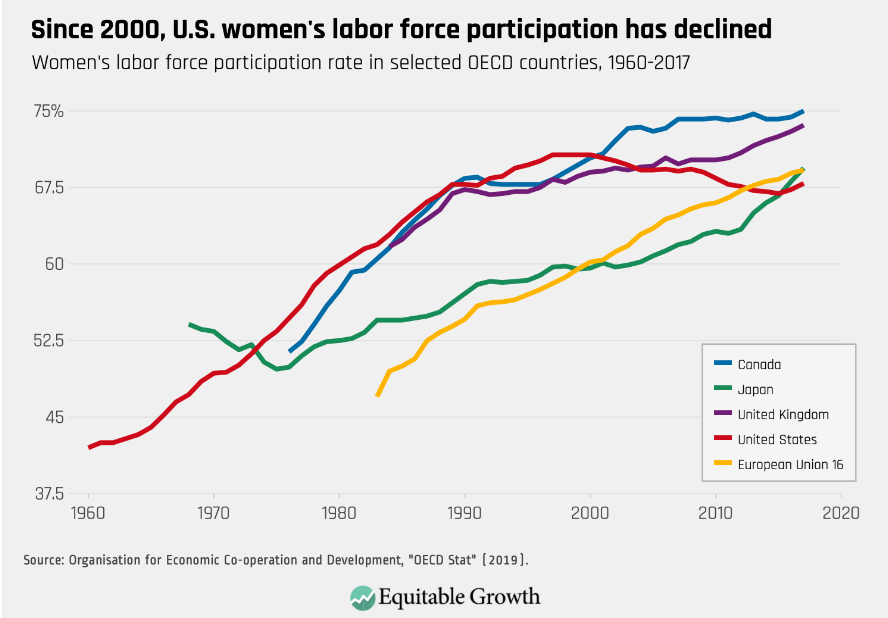
\includegraphics[width = 0.75\textwidth,keepaspectratio]{./figs/since2000.png}
\end{frame}

\begin{frame}{Income and substitution effects}
    \begin{itemize}
        \item Flattening LFPR in recent years suggests these two effects are relatively balanced --- and the income effect may be stronger in the US
        \item Important lesson: economics often involves multiple channels working at the same time, with an \textit{ambiguous} net effect
        \begin{itemize}
            \item In this case, that a wage increase could increase \textit{or} decrease work hours
        \end{itemize}
        \item Important to measure and distinguish between these channels to fully understand what is driving a trend
    \end{itemize}
\end{frame}

\begin{frame}{Conclusion}
    Key takeaways from today:
    \begin{itemize}
        \item Labor economics is a great field and you all should go study it
        \item Claudia Goldin is an incredible scholar
        \item Economics has interesting things to say about the world!
    \end{itemize}

    \vspace{5mm}
    
    \centering
    \large
    Thank you!

\end{frame}


\end{document}